\hypertarget{ed2-corrections}{%
\chapter{Simulation numérique des solutions}\label{ed2-corrections}}

\hypertarget{ed2-correc_consist}{%
\section{Consistance et ordre de schémas}\label{ed2-correc_consist}}

Vu que \(f\) est \(C^2\), la dérivée seconde (en temps) des solutions
s'écrit \begin{align*}
\ddot{x}(t) &= \frac{d}{dt}\Big( f(t,x(t)) \Big) = \partial_t f(t,x(t))+ \partial_x f(t,x(t)) \dot{x}(t)\\ 
&= \partial_t f(t,x(t))+ \partial_x f(t,x(t)) f(t,x(t)).
\end{align*} On a donc \[
f^{[1]}(t,x) = \partial_t f(t,x)+ \partial_x f(t,x) f(t,x)
\] et la formule de Taylor le long des solutions donne \begin{equation}
\label{ed2-eq:DL_sol_exacte}
\begin{aligned}
x(t_{j+1}) = x(t_j) & + {\Delta t}f(t_j,x(t_j)) \\
& + \frac{{\Delta t}^2}{2} \Big( \partial_t f(t_j,x(t_j)) + \partial_x f(t_j,x(t_j)) f(t_j,x(t_j)) \Big) + \mathrm{O}({\Delta t}^3).
\end{aligned}
\end{equation}

Pour les calculs de consistance, deux options possibles:

\begin{itemize}
\item
  soit on compare à la main \eqref{ed2-eq:DL_sol_exacte} aux développements
  en puissances de \({\Delta t}\) de la solution numérique \(x^{j+1}\),
  partant de \(x(t_j)\).
\item
  soit on utilise la
  \protect\hyperlink{ed2-theo_CS_consistance_ordre_p}{condition nécessaire
  et suffisante de consistance (p.
  \pageref*{ed2-theo_CS_consistance_ordre_p})}.
\end{itemize}

\hypertarget{ed2-answer-consist-1}{%
\subsubsection*{Question 1}\label{ed2-answer-consist-1}}

\addcontentsline{toc}{subsubsection}{Question 1}

A la main, pour la méthode de Heun, \[
\eta^{j+1} = \frac{1}{{\Delta t}}\left( x(t_{j+1}) - x(t_j) - \frac{{\Delta t}}{2}\left[ f(t_j,x(t_j)) + f\Big(t_{j+1},x(t_j)+{\Delta t}f(t_j,x(t_j)) \Big) \right]\right). 
\] Or, \[
\begin{aligned}
f\Big(t_{j+1},&x(t_j)+{\Delta t}f(t_j,x(t_j)) \Big)\\ 
&= f(t_j,x(t_j)) +  \partial_t f(t_j,x(t_j))(t_{j+1}-t_j) + \partial_x f(t_j,x(t_j)) {\Delta t}f(t_j,x(t_j)) + \mathrm{O}({\Delta t}^2)\\
& = f(t_j,x(t_j)) + {\Delta t}\Big( \partial_t f(t_j,x(t_j)) + \partial_x f(t_j,x(t_j)) f(t_j,x(t_j)) \Big) + \mathrm{O}({\Delta t}^2).
\end{aligned}
\] On en déduit que \(\eta^{j+1} = \mathrm{O}({\Delta t}^2)\) en
utilisant \eqref{ed2-eq:DL_sol_exacte}. Donc on a une consistance d'ordre
\(\geq 2\).

Sinon il suffit de constater que \[
\Phi(t,x,0) = f(t,x) \quad ,\quad \frac{\partial \Phi}{\partial {\Delta t}}(t,x,0) = \frac{1}{2} f^{[1]}(t,x)   \ .
\] Par contre, si \(f\) est \(C^3\),
\(\frac{\partial^2 \Phi}{\partial {\Delta t}^2}(t,x,0) \neq \frac{1}{3} f^{[2]}(t,x)\)
donc le schéma n'est pas d'ordre 3 et donc il est d'ordre égal
exactement à 2.

\hypertarget{ed2-answer-consist-2}{%
\subsubsection*{Question 2}\label{ed2-answer-consist-2}}

\addcontentsline{toc}{subsubsection}{Question 2}

Pour le schéma d'Euler implicite \[
\eta^{j+1} = \frac{x(t_{j+1}) - x(t_j) - \Delta t f(t_{j+1},x^{j+1})}{{\Delta t}},
\] où \(x^{j+1}\) est solution de \[
x^{j+1} = x(t_j) + {\Delta t}f\left(t_{j+1},x^{j+1}\right).
\] Comme vu dans la section \protect\hyperlink{ed2-sec_def_impl}{Définition
implicite de \(\Phi\) (p. \pageref*{ed2-sec_def_impl})}, cette définition
implicite de \(x^{j+1}\) admet une unique solution pour \({\Delta t}\)
suffisamment petit si \(f\) est Lipschitzienne par rapport à \(x\). On
aimerait dire ici que \(x^{j+1} = x(t_j) + \mathrm{O}({\Delta t})\) pour
\({\Delta t}\) suffisamment petit. Pour faire ça proprement, fixons
\((t_j,x(t_j))\) et posons \[
F(x,{\Delta t}) = x - \big(x(t_j) + {\Delta t}f\left(t_j+{\Delta t},x\right)\big) 
\] qui est de classe \(C^1\). On a alors \[
F(x(t_j),0) = 0 \quad , \quad F(x^{j+1},{\Delta t})=0 \ .
\] Puisque \(\partial_x F(x(t_j),0) = \text{Id}\) est inversible, le
théorème des fonctions implicites nous dit que pour \(\Delta t\)
suffisamment petit, il existe une fonction \(\psi\) de classe \(C^1\)
telle que \[
F(x^{j+1},{\Delta t})=0 \qquad , \qquad x^{j+1} = \psi({\Delta t}) 
\] au voisinage de \((x(t_j),0)\). Puisque \(\psi\) est continue, il
s'ensuit donc bien que \(x^{j+1} = x(t_j) + \mathrm{O}({\Delta t})\). On
a donc \begin{align*}
f(t_{j+1},x^{j+1}) &= f(t_j,x(t_j)) + \partial_t f(t_j,x(t_j)) (t_{j+1}-t_j) +  \partial_x f(t_j,x(t_j))(x^{j+1} - x(t_j)) + \mathrm{O}(\|h\|^2) \\
&= f(t_j,x(t_j)) + \mathrm{O}({\Delta t})
\end{align*} avec l'incrément \(h=(t_{j+1}-t_j,x^{j+1} - x(t_j))\) qui
vérifie \(\|h\|=\mathrm{O}({\Delta t})\).

Ainsi, toujours au vu de \eqref{ed2-eq:DL_sol_exacte}, \[
\eta^{j+1} = \frac{1}{{\Delta t}}\left[ x(t_{j+1}) - \Big( x(t_j) + \Delta t f(t_j,x(t_j)) + \mathrm{O}({\Delta t}^2) \Big) \right]= \mathrm{O}({\Delta t}).
\]

\hypertarget{ed2-answer-consist-3}{%
\subsubsection*{Question 3}\label{ed2-answer-consist-3}}

\addcontentsline{toc}{subsubsection}{Question 3}

Pour la méthode des trapèzes, on a l'erreur \[
\eta^{j+1} = \frac{x(t_{j+1}) - x(t_j) - \frac{{\Delta t}}{2} \left(f(t_j,x(t_j))+ f(t_{j+1},x^{j+1})\right)}{{\Delta t}},
\] où \(x^{j+1}\) est solution de \[
x^{j+1} = x(t_j) + \frac{{\Delta t}}{2} \left(f(t_j,x(t_j))+ f(t_{j+1},x^{j+1})\right) .
\] Cette fois-ci on voudrait montrer que
\(x^{j+1} = x(t_j)+{\Delta t}f(t_j, x(t_j)) + \mathrm{O}({\Delta t}^2)\).
Pour cela, on redéfinit \[
F(x,{\Delta t}) = x - \big(x(t_j) +\frac{{\Delta t}}{2} \left(f(t_j,x(t_j))+ f(t_{j}+{\Delta t},x^{j+1})\right) \big) 
\] qui est de classe \(C^1\). On a alors \[
F(x(t_j),0) = 0 \quad , \quad F(x^{j+1},{\Delta t})=0 \ .
\] Puisque \(\partial_x F(x(t_j),0) = \text{Id}\) est inversible, le
théorème des fonctions implicites nous dit que pour \(\Delta t\)
suffisamment petit, il existe une fonction \(\psi\) de classe \(C^1\)
telle que \[
F(x^{j+1},{\Delta t})=0 \qquad , \qquad x^{j+1} = \psi({\Delta t}) 
\] au voisinage de \((x(t_j),0)\) et de plus, \[
\psi'(0) = \text{Id}^{-1} \cdot \partial_{\Delta t} F(x(t_j),0) = f(t_j,x(t_j)) \ .
\] Puisque \(\psi\) est de classe \(C^1\), on a donc bien \[
x^{j+1} = x(t_j)+{\Delta t}f(t_j, x(t_j)) + \mathrm{O}({\Delta t}^2) \ .
\] Il s'ensuit que \[
f(t_{j+1},x^{j+1}) = f(t_j, x(t_j)) + {\Delta t}\left(\partial_t f(t_j,x(t_j)) + \partial_x f(t_j,x(t_j))f(t_j, x(t_j))\right) + \mathrm{O}({\Delta t}^2)
\] soit \[
x^{j+1} = x(t_j) + {\Delta t}f(t_j,x(t_j) + \frac{{\Delta t}^2}{2} \left(\partial_t f(t_j,x(t_j)) + \partial_x f(t_j,x(t_j))f(t_j, x(t_j))\right) + \mathrm{O}({\Delta t}^3)
\] On en déduit donc \(\eta^{j+1}=\mathrm{O}({\Delta t}^2)\).

\hypertarget{ed2-answer-consist-4}{%
\subsubsection*{Question 4}\label{ed2-answer-consist-4}}

\addcontentsline{toc}{subsubsection}{Question 4}

Enfin, pour la méthode du point milieu, on a l'erreur \[
\eta^{j+1} = \frac{x(t_{j+1}) - x(t_j) - {\Delta t}f\left(t_j+\frac{{\Delta t}}{2},\frac{x(t_j)+x^{j+1}}{2}\right)}{{\Delta t}},
\] où \(x^{j+1}\) est solution de \[
x^{j+1} = x(t_j) + {\Delta t}f\left(t_j+\frac{{\Delta t}}{2},\frac{x(t_j)+x^{j+1}}{2}\right) .
\] On montre de la même façon qu'à la question précédente que pour
\({\Delta t}\) suffisamment petit,
\(x^{j+1} = x(t_j)+{\Delta t}f(t_j, x(t_j)) + \mathrm{O}({\Delta t}^2)\)
et donc \begin{align*}
f&\left(t_j+\frac{{\Delta t}}{2},\frac{x(t_j)+x^{j+1}}{2}\right)\\ &= f(t_j,x(t_j)) + \partial_t f(t_j,x(t_j)) \frac{{\Delta t}}{2} +  \partial_x f(t_j,x(t_j))\left(\frac{x(t_j)+x^{j+1}}{2} - x(t_j)\right) + \mathrm{O}(\|h\|^2) \\
&= f(t_j, x(t_j)) + \frac{{\Delta t}}{2} (\partial_t f(t_j,x(t_j)) + \partial_x f(t_j,x(t_j))f(t_j,x(t_j))) + \mathrm{O}({\Delta t}^2)
\end{align*} avec l'incrément
\(h=\left(\frac{{\Delta t}}{2}, \frac{x(t_j)+x^{j+1}}{2} - x(t_j)\right)\),
soit \[
x^{j+1} = x(t_j) + {\Delta t}f(t_j,x(t_j) + \frac{{\Delta t}^2}{2} (\partial_t f(t_j,x(t_j)) + \partial_x f(t_j,x(t_j))f(t_j,x(t_j))) + \mathrm{O}({\Delta t}^3)
\] On en déduit donc \(\eta^{j+1}=\mathrm{O}({\Delta t}^2)\).

\hypertarget{ed2-answer-consist-5}{%
\subsubsection*{Question 5}\label{ed2-answer-consist-5}}

\addcontentsline{toc}{subsubsection}{Question 5}

On vérifie que le critère est vérifié pour \(0\leq k \leq 3\) mais pas
pour \(k=4\)\,!

\hypertarget{ed2-answer-conv}{%
\section{Convergence de schémas}\label{ed2-answer-conv}}

Tout d'abord, dans l'exercice précédent, nous avons montré que les
schémas de Heun et d'Euler implicite étaient consistants d'ordre 2 et 1
respectivement. Il ne nous reste donc plus qu'à montrer que \(\Phi\) est
localement lipschitzienne (ou \(C^1\)) par rapport à \(x\) pour
\({\Delta t}\) suffisamment petit, pour en déduire la convergence à
l'ordre 2 et 1 respectivement.

Pour le schéma de Heun, \[
\Phi(t,x,{\Delta t}) = \frac{1}{2}\Big(f(t,x) + f\big(t+{\Delta t},x+{\Delta t}f(t,x)\big)\Big)
\] donc \(\Phi\) est \(C^1\) par rapport à \(x\) si \(f\) l'est.

Prenons maintenant le schéma d'Euler implicite. Pour
\({\Delta t}\leq {\Delta t}_m\), \(\Phi\) est définie par \[
\Phi(t,x,{\Delta t}) = f\Big(t+ {\Delta t}, x + {\Delta t}\Phi(t,x,{\Delta t}) \Big).
\] Soit \(B\) un compact de \(\mathbb{R}^n\). Soit \(B'\) un compact tel
que \(x + {\Delta t}\Phi(t,x,{\Delta t}) \in B'\) pour tout \(x\in B\),
tout \(t\in [ 0,T ]\) et tout \({\Delta t}\in [ 0,{\Delta t}_m ]\).
Puisque \(f\) est continue, et \(C^1\) par rapport à \(x\), il existe
\(L_f>0\) tel que \[
\|f(t,x_a) - f(t,x_b) \| \leq L_f \|x_a-x_b\| \qquad \forall (x_a,x_b,t)\in B'\times B' \times [ 0,T+{\Delta t}_m ] \ . 
\] Ceci est vrai par le théorème des accroissements finis appliqué à
\(x\mapsto f(t,x)\) et pour \(t\) dans un intervalle fermé et borné.
Prenons maintenant \((x_a,x_b)\in B\times B\), \(t\in [ 0,T ]\) et
\({\Delta t}\in [ 0,{\Delta t}_m ]\), alors \begin{align*}
\|&\Phi(t,x_a,{\Delta t})-\Phi(t,x_b,{\Delta t}) \|\\ &= \| f\Big(t+ {\Delta t}, x_a + {\Delta t}\Phi(t,x_a,{\Delta t}) \Big)-f\Big(t+ {\Delta t}, x_b + {\Delta t}\Phi(t,x_b,{\Delta t}) \Big) \|\\
&\leq L_f \left( \|x_a-x_b \| + {\Delta t}\|\Phi(t,x_a,{\Delta t})-\Phi(t,x_b{\Delta t}) \| \right)
\end{align*} soit \[
\|\Phi(t,x_a,{\Delta t})-\Phi(t,x_b,{\Delta t}) \| \leq \frac{L_f}{1-L_f {\Delta t}} \|x_a-x_b \|
\] si \({\Delta t}< 1/L_f\). Donc \(\Phi\) est bien localement
lipschitzienne par rapport à \(x\).

\hypertarget{ed2-explicite-ou-implicite}{%
\section{Explicite ou implicite\,?}\label{ed2-explicite-ou-implicite}}

\hypertarget{ed2-answer-impl-1}{%
\subsubsection*{Question 1}\label{ed2-answer-impl-1}}

\addcontentsline{toc}{subsubsection}{Question 1}

Prenons d'abord \(\dot{x}= -\lambda x\), \(x(0)=1\), dont la solution
exacte est \(x(t)=e^{-\lambda t}\).

Le schéma d'Euler explicite donne \[
x^{j+1} = x^j - \lambda{\Delta t}x^j =(1-\lambda{\Delta t})^j
\] soit \[
x^{J} = (1-\lambda{\Delta t})^J = (1-\lambda{\Delta t})^{\frac{T}{{\Delta t}}} = \left((1-\lambda{\Delta t})^{\frac{T}{\lambda{\Delta t}}} \right)^\lambda \ .
\] On a bien \[
\lim_{{\Delta t}\to 0} x^{J} = e^{-\lambda T} \ .
\] Cependant, il faut \(|1-\lambda{\Delta t}|<1\) pour que la solution
converge au moins vers 0. Sinon, pour \(\lambda{\Delta t}= 2\),
\(x^J = (-1)^J\), qui n'a rien à voir avec la solution. Pire, pour
\(\lambda{\Delta t}= 2\), l'algorithme diverge. Il faut donc adapter
\({\Delta t}\) à la constante de temps \(\lambda\) du système. Ceci peut
poser problème lorsque l'on simule des systèmes sur des temps longs (par
rapport à \(\lambda\))

De l'autre côté, le schéma d'Euler implicite donne \[
x^{j+1} = x^j - \lambda{\Delta t}x^{j+1} 
\] soit \[
x^J = \frac{1}{(1+\lambda {\Delta t})^J} =  \frac{1}{(1+\lambda {\Delta t})^\frac{T}{{\Delta t}}}
\] qui tend vers 0 quelque soit le pas \({\Delta t}\)\,! On parle de
stabilité inconditionnelle. Ceci est très pratique pour des simulations
sur temps longs, où la condition \(\lambda{\Delta t}<1\) est trop
contraignante.

Prenons maintenant \(\dot{x}= \lambda x\), \(x(0)=1\), dont la solution
exacte est \(x(t)=e^{\lambda t}\). Cette fois-ci, Euler explicite donne
\[
x^{J} = (1+\lambda{\Delta t})^{\frac{T}{{\Delta t}}}
\] qui fait maintenant sens même pour des pas grands. Par contre, Euler
implicite donne \[
x^J =   \frac{1}{(1-\lambda {\Delta t})^\frac{T}{{\Delta t}}}
\] qui n'est pas défini pour \(\lambda {\Delta t}=1\) et qui explose
pour des valeurs proche de 1.

\hypertarget{ed2-answer-impl-2}{%
\subsubsection*{Question 2}\label{ed2-answer-impl-2}}

\addcontentsline{toc}{subsubsection}{Question 2}

Lorsque l'on a deux dynamiques asymptotiquement stables aux constantes
de temps très différentes la condition de stabilité de Euler explicite
exige de choisir un pas câlé sur la plus petite constante de temps,
i.e.~il faut \({\Delta t}<\frac{1}{\mu}\). Ceci est très exigeant car il
faut attendre un nombre d'itérations de l'ordre de \(\mu\) pour voir
l'évolution du système lent. Par contre, une méthode implicite permet de
choisir librement le pas de temps en fonction des performances
souhaitées.

\hypertarget{ed2-answer-impl-3}{%
\subsubsection*{Question 3 (Frottement sec)}\label{ed2-answer-impl-3}}

\addcontentsline{toc}{subsubsection}{Question 3}

\begin{enumerate}
\def\labelenumi{\alph{enumi})}
\item
  Tant que \(x(t)>0\), l'équation s'écrit \(\dot{x}=-1\), donc
  \(x(t) = x_0 - t\)\,: ceci est valable jusqu'à l'instant
  \(t^* = x_0\) où \(x\) s'annule. Ensuite, \(x\equiv 0\) est solution
  puisque \(\mathrm{sign}(0)=0\), et c'est la seule continuation qui
  reste continue et vérifie l'équation\,: si \(x\) redevenait strictement
  positive (resp. négative) sur un intervalle, on y aurait
  \(\dot x = -1\) (resp. \(+1\)), ce qui ramène vers 0. Par symétrie,
  pour tout \(x_0\), \[
  x(t) = \begin{cases} x_0 - \mathrm{sign}(x_0)\, t & \text{si } t\leq t^* := |x_0| \\ 0 & \text{si } t\geq t^* \end{cases}
  \] qui est continue, dérivable sauf en \(t^*\), et vérifie l'équation
  partout ailleurs. Contrairement à \(e^{-\lambda t}\), qui ne s'annule
  jamais, la solution \emph{atteint exactement l'équilibre en temps fini}
  et y reste\,: un solide freiné par frottement sec s'arrête, alors
  qu'un solide freiné par frottement visqueux ralentit indéfiniment.

  Ceci est impossible pour \(f\) continûment différentiable (ou
  seulement localement Lipschitzienne)\,: le théorème de
  Cauchy-Lipschitz garantit alors l'unicité des solutions, y compris en
  temps rétrograde. Si une solution atteignait l'équilibre \(x^*\) en un
  temps \(t^*\), elle coïnciderait, par unicité de la solution passant par
  \((t^*,x^*)\), avec la solution stationnaire \(x\equiv x^*\), donc on
  aurait \(x(0)=x^*\). La convergence en temps fini est un phénomène
  propre aux dynamiques non Lipschitziennes.
\item
  Le schéma d'Euler explicite s'écrit \[
  x^{j+1} = x^j - {\Delta t}\, \mathrm{sign}(x^j) \ .
  \] Partant de \(x_0>0\), la suite décroît de \({\Delta t}\) à chaque
  pas, \(x^j = x_0 - j{\Delta t}\), tant que \(x^j>0\). Soit \(J\) le
  premier indice tel que \(x^J\leq 0\), c'est-à-dire \(x^{J-1}\in \left]0,{\Delta t}\right]\)
  et \(x^J = x^{J-1}-{\Delta t}\in\left]-{\Delta t},0\right]\). Si par
  chance \(x^J=0\) (i.e. \(x_0\) est un multiple de \({\Delta t}\)), la
  suite y reste. Sinon \(x^J<0\) et \(x^{J+1} = x^J + {\Delta t} = x^{J-1}>0\),
  puis \(x^{J+2} = x^J<0\), etc.\,: la suite est \(2\)-périodique et
  \emph{oscille indéfiniment} entre \(x^{J-1}>0\) et \(x^J<0\), avec une
  amplitude \({\Delta t}\), à la fréquence maximale que permet le pas. Ce
  phénomène est appelé \emph{chattering}. Diminuer \({\Delta t}\) réduit
  l'amplitude des oscillations mais ne les supprime pas\,: la solution
  numérique ne s'arrête jamais, et sa ``vitesse'' \((x^{j+1}-x^j)/{\Delta t}\)
  vaut \(\pm 1\) alors que la vraie vaut 0. Le comportement
  est qualitativement faux pour tout \({\Delta t}>0\) (et en pratique
  catastrophique si \(\mathrm{sign}(x)\) pilote une force\,: celle-ci
  change de sens à chaque pas).
\item
  Le schéma d'Euler implicite s'écrit \[
  x^{j+1} = x^j - {\Delta t}\, \mathrm{sign}(x^{j+1}) \ .
  \] Raisonnons par disjonction des cas sur le signe de \(x^{j+1}\)\,:

  \begin{itemize}
  \tightlist
  \item
    si \(x^{j+1}>0\), alors \(x^{j+1} = x^j - {\Delta t}\), ce qui exige
    \(x^j>{\Delta t}\)\,;
  \item
    si \(x^{j+1}<0\), alors \(x^{j+1} = x^j + {\Delta t}\), ce qui exige
    \(x^j<-{\Delta t}\)\,;
  \item
    si \(x^{j+1}=0\), alors \(0 = x^j - {\Delta t}\,\mathrm{sign}(0)\),
    soit \(x^j = 0\) avec la convention \(\mathrm{sign}(0)=0\).
  \end{itemize}

  Pour \(0<|x^j|\leq {\Delta t}\), aucun des trois cas n'est possible\,:
  l'équation n'a pas de solution, et le schéma implicite n'est pas
  défini. La convention \(\mathrm{sign}(0)=0\) est trop restrictive\,: si
  l'on autorise \(\mathrm{sign}(0)\) à prendre n'importe quelle valeur
  \(s\in[-1,1]\), le troisième cas devient \(x^j = {\Delta t}\, s\),
  possible exactement lorsque \(|x^j|\leq {\Delta t}\), avec
  \(s = x^j/{\Delta t}\). Les trois cas sont alors mutuellement exclusifs
  et recouvrent toutes les valeurs de \(x^j\)\,: pour tout \(x^j\),
  l'équation implicite a une unique solution \[
  x^{j+1} = \begin{cases} x^j - {\Delta t} & \text{si } x^j > {\Delta t} \\ 0 & \text{si } |x^j|\leq {\Delta t} \\ x^j + {\Delta t} & \text{si } x^j < -{\Delta t} \end{cases}
  \qquad \text{i.e.} \qquad x^{j+1} = \mathrm{sign}(x^j)\max\big(|x^j| - {\Delta t},\, 0\big) \ .
  \] Autoriser \(\mathrm{sign}(0)\in[-1,1]\) n'est pas un artifice\,:
  physiquement, le frottement sec à l'arrêt prend exactement la valeur
  nécessaire pour compenser les autres forces, dans la limite de son
  module maximal\,; mathématiquement, c'est la définition des solutions
  au sens de Filippov des équations à second membre discontinu (voir la
  remarque \emph{Classe plus générale de solutions} du chapitre I).
\item
  Partant de \(x_0>0\), la suite implicite est \(x^j = \max(x_0 - j{\Delta t}, 0)\)\,:
  elle décroît de \({\Delta t}\) par pas, atteint \emph{exactement} 0 au
  premier indice \(J\) tel que \(J{\Delta t}\geq x_0\), et y reste. Elle
  coïncide avec la solution exacte aux instants \(t_j\) pour \(t_j\leq t^*\),
  et ensuite à une erreur près d'au plus \({\Delta t}\) sur l'instant
  d'arrêt\,: il n'y a plus de chattering, et ce quel que soit le pas
  \({\Delta t}\) (même très grand). Le schéma implicite reproduit le
  comportement qualitatif de la solution, l'arrêt en temps fini, que le
  schéma explicite est incapable de produire. 
%  Pour le voir, écrivons les
%  deux schémas sous la forme \(\Psi(x^{j+1}) = x^j\) ou \(x^{j+1} = \Phi(x^j)\) avec \[
%  \Psi(x) = x + {\Delta t}\,\mathrm{sign}(x) \qquad , \qquad \Phi(x) = x - {\Delta t}\,\mathrm{sign}(x) \ .
%  \] L'application \(\Psi\) est \emph{strictement croissante} (avec
%  \(\mathrm{sign}(0)\in[-1,1]\), son graphe est une courbe croissante qui
%  saute de \(-{\Delta t}\) à \({\Delta t}\) en 0)\,: elle est injective et
%  atteint toutes les valeurs, donc \(x^{j+1}=\Psi^{-1}(x^j)\) est bien
%  défini et unique, et \(\Psi^{-1}\) est continue, croissante, et
%  ``écrase'' tout l'intervalle \([-{\Delta t},{\Delta t}]\) sur 0.
%  L'application \(\Phi\), au contraire, n'est pas monotone\,: elle
%  envoie \(\left]0,{\Delta t}\right]\) sur \(\left]-{\Delta t},0\right]\)
%  et réciproquement, d'où l'oscillation. C'est le même mécanisme que
%  pour \(\dot{x} = -\lambda x\) avec \(\lambda{\Delta t}>2\) (question
%  1)\,: le schéma implicite inverse une application monotone
%  \(x\mapsto x+{\Delta t}\lambda x\), ce qui est toujours possible et
%  contractant, alors que l'explicite applique \(x\mapsto x - {\Delta t}\lambda x\)
%  qui change de signe. La discontinuité joue ici le rôle d'une raideur
%  infinie. 
  Les deux comportements sont comparés sur la
  \protect\hyperlink{ed2-fig_frottement_sec}{Figure~\ref*{ed2-fig_frottement_sec}
  (p. \pageref*{ed2-fig_frottement_sec})}.
\end{enumerate}

\begin{figure}
\hypertarget{ed2-fig_frottement_sec}{%
\centering
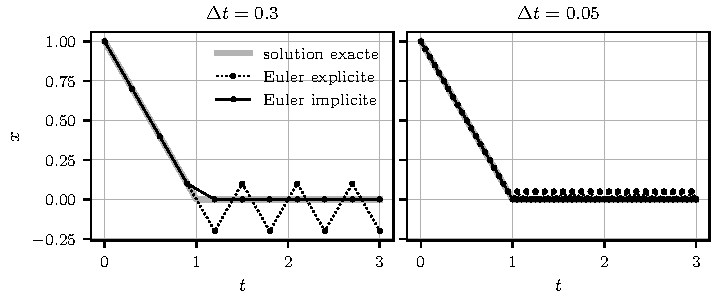
\includegraphics[width=\linewidth]{images/frottement_sec.py.pdf}
\caption{Simulation de \(\dot{x}=-\mathrm{sign}(x)\), \(x(0)=1\), par
les schémas d'Euler explicite et implicite avec \({\Delta t}=0{,}3\)
(à gauche) et \({\Delta t}=0{,}05\) (à droite). Le schéma explicite
oscille indéfiniment autour de 0 avec une amplitude \({\Delta t}\)
(chattering)\,; le schéma implicite s'arrête exactement en 0. 
%Le code
%générant cette figure est
%\texttt{images/frottement\_sec.py}.
}\label{ed2-fig_frottement_sec}
}
\end{figure}

\hypertarget{ed2-euler-symplectique}{%
\section{Euler symplectique}\label{ed2-euler-symplectique}}

\hypertarget{ed2-answer-symp-1}{%
\subsubsection*{Question 1}\label{ed2-answer-symp-1}}

\addcontentsline{toc}{subsubsection}{Question 1}

Dans le cas d'Euler explicite, \(x^{j+1}=Ax^j\) avec \[
A = \left(
\begin{matrix}
1 & {\Delta t}\\
-{\Delta t}\, \omega^2 & 1
\end{matrix}
\right)
\] dont les valeur propres sont \(1 \pm i\omega {\Delta t}\) de norme
\(\sqrt{1+{\Delta t}^2 \, \omega^2}>1\). Donc les solutions divergent.

Dans le cas d'Euler implicite, \(x^{j+1}=Ax^j\) avec \[
A = \frac{1}{1+{\Delta t}^2 \, \omega^2} \left(
\begin{matrix}
1 & {\Delta t}\\
-{\Delta t}\, \omega^2 & 1
\end{matrix}
\right)
\] dont les valeurs propres sont \(1/(1 \pm i\omega {\Delta t})\) de
norme \(1/\sqrt{1+{\Delta t}^2 \, \omega^2}<1\). Donc les solutions
convergent vers 0.

Or on peut vérifier que le long des vraies solutions, l'énergie
\(\omega^2 x_1^2 + x_2^2\) est constante donc les trajectoires sont
bornées et ne peuvent pas converger vers zéro. Aucun des deux schémas
n'approxime les solutions correctement sur le long-terme.

\hypertarget{ed2-answer-symp-2}{%
\subsubsection*{Question 2}\label{ed2-answer-symp-2}}

\addcontentsline{toc}{subsubsection}{Question 2}

Le schéma symplectique donne \[
\left( 
  \begin{matrix}
  \omega^2 & 0 \\
  {\Delta t}\, w^2 & 1
  \end{matrix}
\right)
\left( 
  \begin{matrix}
  x_1^{j+1}\\
  x_2^{j+1}
  \end{matrix}
\right)
=
\left( 
  \begin{matrix}
  \omega^2 & {\Delta t}\, w^2 \\
  0 & 1
  \end{matrix}
\right)
\left( 
  \begin{matrix}
  x_1^{j}\\
  x_2^{j}
  \end{matrix}
\right)
\] En multipliant à gauche alternativement par
\(\left( \begin{matrix}x_1^{j+1} & x_2^{j+1}\end{matrix}\right)\) et
\(\left( \begin{matrix}x_1^{j} & x_2^{j}\end{matrix}\right)\), on
obtient \begin{align*}
\omega^2 (x_1^{j+1})^2 + (x_2^{j+1})^2 +{\Delta t}\, \omega^2 x_1^{j+1}x_2^{j+1}
&= \omega^2 x_1^{j+1} x_1^j + x_2^{j+1}x_2^j +{\Delta t}\, \omega^2 x_1^{j+1}x_2^{j} \\
&= \omega^2 (x_1^{j})^2 + (x_2^{j})^2 +{\Delta t}\, \omega^2 x_1^{j}x_2^{j} 
\end{align*} et donc la quantité
\(\omega^2 x_1^2 + x_2^2 +{\Delta t}\, \omega^2 x_1x_2\) est bien
constante. Pour \(\omega^2-\frac{{\Delta t}^2 \omega^4}{4}>0\), soit
\(\omega {\Delta t}<2\), cette matrice est définie positive, donc les
solutions restent sur une ellipse. Cette ellipse se rapproche de la
vraie solution lorsque \({\Delta t}\) tend vers 0. Ce schéma est donc
approprié pour simuler les trajectoires sur un temps long. Les trois
schémas sont comparés sur la
\protect\hyperlink{ed2-fig_oscillateur_symplectique}{Figure~\ref*{ed2-fig_oscillateur_symplectique}
(p. \pageref*{ed2-fig_oscillateur_symplectique})}\,: en quelques
périodes, Euler explicite spirale vers l'extérieur et Euler implicite
vers l'origine, tandis qu'Euler symplectique reste sur une ellipse proche
du cercle exact. Son énergie \(\omega^2 x_1^2 + x_2^2\) n'est pas
exactement constante, mais oscille sans dériver\,; c'est la quantité
modifiée \(\omega^2 x_1^2 + x_2^2 +{\Delta t}\, \omega^2 x_1x_2\) qui
est conservée.

\begin{figure}
\hypertarget{ed2-fig_oscillateur_symplectique}{%
\centering
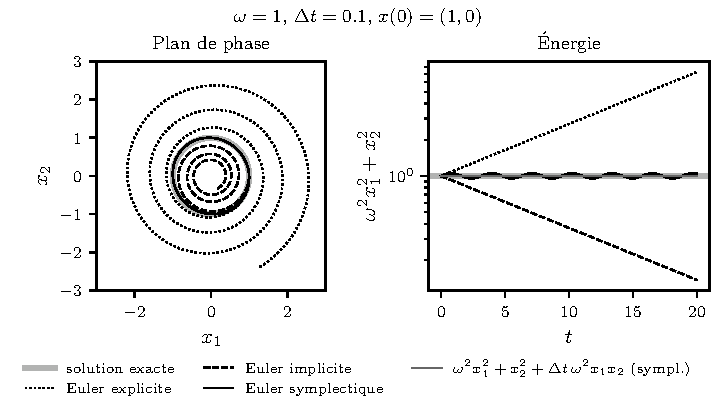
\includegraphics[width=\linewidth]{images/oscillateur_symplectique.py.pdf}
\caption{Simulation de l'oscillateur \(\dot x_1 = x_2\),
\(\dot x_2 = -\omega^2 x_1\) par les schémas d'Euler explicite, implicite
et symplectique (\(\omega=1\), \({\Delta t}=0{,}1\), trois périodes). 
%A gauche, le plan de phase\,; à droite, l'énergie \(\omega^2 x_1^2 + x_2^2\) le long des solutions numériques, en échelle logarithmique. Le code générant cette figure est \texttt{images/oscillateur\_symplectique.py}.
}\label{ed2-fig_oscillateur_symplectique}
}
\end{figure}

\hypertarget{ed2-answer-symp-3}{%
\subsubsection*{Question 3}\label{ed2-answer-symp-3}}

\addcontentsline{toc}{subsubsection}{Question 3}

L'algorithme symplectique est décrit par \(x^{j+1}=Ax^j\) avec \[
A = \left(
\begin{matrix}
1 & {\Delta t}\\
-{\Delta t}\, \omega^2 & 1-{\Delta t}^2 \, \omega^2
\end{matrix}
\right)
\] dont le polynôme caractéristique s'écrit \[
s^2 - (2-{\Delta t}^2 \, \omega^2) s + 1
\] On a les cas suivants~:

\begin{itemize}
\item
  si \((2-{\Delta t}^2 \, \omega^2)^2 -4 <0\), i.e., si
  \(\omega {\Delta t}<2\), les valeurs propres sont imaginaires
  conjuguées et de module 1.
\item
  si \(\omega {\Delta t}> 2\), les valeurs propres sont réelles de
  produit 1, donc l'une est supérieure à 1 est le schéma diverge.
\item
  dans le cas extrême où \(\omega {\Delta t}= 2\), il y a une valeur
  propre double en -1.
\end{itemize}

\hypertarget{ed2-answer-symp-4}{%
\subsubsection*{Question 4}\label{ed2-answer-symp-4}}

\addcontentsline{toc}{subsubsection}{Question 4}

Pour un système hamiltonien, on peut donc proposer \begin{align*}
q^{j+1} &= q^{j} + {\Delta t}\, \nabla_p H(q^{j},p^{j}) \\
p^{j+1} &= p^{j} - {\Delta t}\, \nabla_q H(q^{j+1},p^{j+1})
\end{align*} ou bien \begin{align*}
q^{j+1} &= q^{j} + {\Delta t}\, \nabla_p H(q^{j+1},p^{j+1}) \\
p^{j+1} &= p^{j} - {\Delta t}\, \nabla_q H(q^{j},p^j)
\end{align*} pour \({\Delta t}\) suffisamment petit. C'est cet algorithme qui est utilis\'e dans la \protect\hyperlink{ed2-fig_systeme_solaire}{Figure~\ref*{ed2-fig_systeme_solaire} (p.
\pageref*{ed2-fig_systeme_solaire})}

